%%%%%%%%%%%%%%%%%%%%%%%%%%%%%%%%%%%%%%%%%
% Arsclassica Article
% LaTeX Template
% Version 1.1 (10/6/14)
%
% This template has been downloaded from:
% http://www.LaTeXTemplates.com
%
% Original author:
% Lorenzo Pantieri (http://www.lorenzopantieri.net) with extensive modifications by:
% Vel (vel@latextemplates.com)
%
% License:
% CC BY-NC-SA 3.0 (http://creativecommons.org/licenses/by-nc-sa/3.0/)
%
%%%%%%%%%%%%%%%%%%%%%%%%%%%%%%%%%%%%%%%%%

%----------------------------------------------------------------------------------------
%	PACKAGES AND OTHER DOCUMENT CONFIGURATIONS
%----------------------------------------------------------------------------------------

\documentclass[
10pt, % Main document font size
a4paper, % Paper type, use 'letterpaper' for US Letter paper
oneside, % One page layout (no page indentation)
%twoside, % Two page layout (page indentation for binding and different headers)
headinclude,footinclude, % Extra spacing for the header and footer
BCOR5mm, % Binding correction
]{scrartcl}

%%%%%%%%%%%%%%%%%%%%%%%%%%%%%%%%%%%%%%%%%
% Arsclassica Article
% Structure Specification File
%
% This file has been downloaded from:
% http://www.LaTeXTemplates.com
%
% Original author:
% Lorenzo Pantieri (http://www.lorenzopantieri.net) with extensive modifications by:
% Vel (vel@latextemplates.com)
%
% License:
% CC BY-NC-SA 3.0 (http://creativecommons.org/licenses/by-nc-sa/3.0/)
%
%%%%%%%%%%%%%%%%%%%%%%%%%%%%%%%%%%%%%%%%%

%----------------------------------------------------------------------------------------
%	REQUIRED PACKAGES
%----------------------------------------------------------------------------------------

\usepackage[
nochapters, % Turn off chapters since this is an article        
beramono, % Use the Bera Mono font for monospaced text (\texttt)
eulermath,% Use the Euler font for mathematics
pdfspacing, % Makes use of pdftex’ letter spacing capabilities via the microtype package
dottedtoc % Dotted lines leading to the page numbers in the table of contents
]{classicthesis} % The layout is based on the Classic Thesis style

\usepackage{arsclassica} % Modifies the Classic Thesis package
\usepackage{siunitx} % SI unit package
\usepackage{bm} % Bold symbols in formulas

\usepackage[T1]{fontenc} % Use 8-bit encoding that has 256 glyphs

\usepackage[utf8]{inputenc} % Required for including letters with accents

\usepackage{graphicx} % Required for including images
\graphicspath{{Figures/}} % Set the default folder for images

\usepackage{enumitem} % Required for manipulating the whitespace between and within lists

\usepackage{lipsum} % Used for inserting dummy 'Lorem ipsum' text into the template

\usepackage{subfig} % Required for creating figures with multiple parts (subfigures)

\usepackage{amsmath,amssymb,amsthm} % For including math equations, theorems, symbols, etc

\usepackage{varioref} % More descriptive referencing

\usepackage{braket} % For dirac notation

% \usepackage{commath} % For differential equations 
%----------------------------------------------------------------------------------------
%	THEOREM STYLES
%---------------------------------------------------------------------------------------

\theoremstyle{definition} % Define theorem styles here based on the definition style (used for definitions and examples)
\newtheorem{definition}{Definition}

\theoremstyle{plain} % Define theorem styles here based on the plain style (used for theorems, lemmas, propositions)
\newtheorem{theorem}{Theorem}

\theoremstyle{remark} % Define theorem styles here based on the remark style (used for remarks and notes)

%----------------------------------------------------------------------------------------
%	HYPERLINKS
%---------------------------------------------------------------------------------------

\hypersetup{
%draft, % Uncomment to remove all links (useful for printing in black and white)
colorlinks=true, breaklinks=true, bookmarks=true,bookmarksnumbered,
urlcolor=webbrown, linkcolor=RoyalBlue, citecolor=webgreen, % Link colors
pdftitle={}, % PDF title
pdfauthor={\textcopyright}, % PDF Author
pdfsubject={}, % PDF Subject
pdfkeywords={}, % PDF Keywords
pdfcreator={pdfLaTeX}, % PDF Creator
pdfproducer={LaTeX with hyperref and ClassicThesis} % PDF producer
}
 % Include the structure.tex file which specified the document structure and layout

\hyphenation{Fortran hy-phen-ation} % Specify custom hyphenation points in words with dashes where you would like hyphenation to occur, or alternatively, don't put any dashes in a word to stop hyphenation altogether

%----------------------------------------------------------------------------------------
%	TITLE AND AUTHOR(S)
%----------------------------------------------------------------------------------------

\title{\normalfont\spacedallcaps{Monte Carlo and Molecular Dynamics Simulation}} % The article title

\author{\spacedlowsmallcaps{William Janke\textsuperscript{1} \& Andreas Haller\textsuperscript{2}}} % The article author(s) - author affiliations need to be specified in the AUTHOR AFFILIATIONS block

\date{} % An optional date to appear under the author(s)

%----------------------------------------------------------------------------------------

\begin{document}

%----------------------------------------------------------------------------------------
%	HEADERS
%----------------------------------------------------------------------------------------

\renewcommand{\sectionmark}[1]{\markright{\spacedlowsmallcaps{#1}}} % The header for all pages (oneside) or for even pages (twoside)
%\renewcommand{\subsectionmark}[1]{\markright{\thesubsection~#1}} % Uncomment when using the twoside option - this modifies the header on odd pages
\lehead{\mbox{\llap{\small\thepage\kern1em\color{halfgray} \vline}\color{halfgray}\hspace{0.5em}\rightmark\hfil}} % The header style

\pagestyle{scrheadings} % Enable the headers specified in this block

%----------------------------------------------------------------------------------------
%	TABLE OF CONTENTS & LISTS OF FIGURES AND TABLES
%----------------------------------------------------------------------------------------

\maketitle % Print the title/author/date block

\setcounter{tocdepth}{2} % Set the depth of the table of contents to show sections and subsections only

\tableofcontents % Print the table of contents

\listoffigures % Print the list of figures

\listoftables % Print the list of tables

%----------------------------------------------------------------------------------------
%	AUTHOR AFFILIATIONS
%----------------------------------------------------------------------------------------

{\let\thefootnote\relax\footnotetext{\textsuperscript{1} \textit{wjanke@students.uni-mainz.de}}}

{\let\thefootnote\relax\footnotetext{\textsuperscript{2} \textit{ahaller@students.uni-mainz.de}}}

%----------------------------------------------------------------------------------------

\newpage\clearpage % Start the article content on the second page, remove this if you have a longer abstract that goes onto the second page

\section{Introduction}
Many body problems often cannot be resolved analytically because of their huge amount of accessible states, for an instance.
In order to solve such a problem with computational assistance, a variety of methods have been developed and all of them have their very own applications and limits.
One of the first models is the Monte Carlo simulation with the Metropolis Criterion.
Its nature is pure stochastic - the time progression evolves randomly and is not given a set of initial conditions.
% The timeframe of its creation is the 1950's during the Manhatten Project by Stanislav Ulam\footnote{$^*$April 13, 1909, $^\dag$May 13, 1984. Ulam got the idea of the MC approach indirectly while he was thinking about the probability of the popular game Solitaire's successful outcome.} and Jan Von Neumann\footnote{$^*$December 28, 1903, $^\dag$February 8, 1957.}.
However, the Molecular Dynamics approach is used for the same initial System - with equal coordinate initialisation and boundary conditions - by solving Newton's equations of motions to all atoms simultaniously.
This implies that this kind of simulations are deterministic and can be used to look into a system's time evolution.\medskip\\
The main goal of this work is an implementation of both methods in C++ for a set of noninteracting particles in a finite box with periodic boundary conditions and Lennard-Jones Potential.
In order to deepen the similarities and differences in computational and physical aspects, a comparison at the very end is suffitient.

\section{System Considerations}
If not explicitly mentioned, the system's settings are as follows:
\subsubsection*{Ensemble}
$N$ particles in a box of volume $V$ and temperature $T$ are considered.
The closed box is placed in an external heat bath, hence the total energy is not fixed and the probability $P_i$ for a given State $\ket{i}$ with Energy $E_i$ and $\beta \mathrel{\mathop:}= \frac{1}{kT}$ is given by
\begin{align}
	P_i = \frac{1}{Z}\exp\left(-\beta E_i\right)\text{, and }
	Z = \sum_k \exp\left(-\beta E_k\right).
\end{align}
Such an ensemble is called canonical or NVT.

\subsubsection*{Potential and Energy}
The particles are interacting via a normed Lennard-Jones Potential
\begin{align}
	V_{ij} = 4\left(\frac{1}{r_{ij}^{12}} - \frac{1}{r_{ij}^6} + \frac{2^7 - 1}{2^{14}}\right),
\end{align}
such that $V_{ij}=0$, if $r_{ij} = 2\sqrt[6]2$.
The total energy $E_n$ of the system in a state $\ket{n}$ is given by the expression
\begin{align}
	E_n = \sum_i\sum_{j\neq i}V_{ij}.
\end{align}

\subsubsection*{Boundary Conditions}
For both implementations, periodic boundary conditions (PBC) will be used.
More detailed - the particles at the border of the box can interact with fake neighbour particles beyond the scope of the border.
To understand the principle of this condition, a simple example is sufficient: Consider a one dimensional chain with next-neighbour interacting particles at fixed lattice points.
Each one has exactly two neighbours, except for the two at the border.
This incident can be terminated when telling the border particles to interact with one another.
This yields a positive effect on the system's scale parameters - box length $L$ and number of particles $N$ - they are implicitely bigger without the need for significantly more calculation steps.

\section{Monte Carlo Simulation}
It has been already mentioned, that MC approaches can be used to research many body systems which are not solvable analytically.
Numerical methods simplify this task, but they introduce other challenges - in most cases (especially for large scaling sizes), it is not possible to acces every single state.
However, for the explanation of the used algorithm, this can be neglected for now.

\subsection{Detailed Balance and the Metropolis Algorithm}
Consider the particle flow out of state $\ket{i}$
\begin{align}
	j^\text{out}_{i} \mathrel{\mathop:}= \sum_j P_i(t) W_{ij},
\end{align}
with jump probability $W_{ij}$ from state $\ket{i}$ to $\ket{j}$.
Analogue, the particle flow into state $\ket{i}$ can be written as
\begin{align}
	j^\text{in}_{i} \mathrel{\mathop:}= \sum_j P_j(t) W_{ji}.
\end{align}
This yields to the master equation
\begin{align}
	\frac{\mathrm{d}P_i(t)}{\mathrm{d}t} = 
		\sum_{j}\left(P_j(t)W_{ji} - P_i(t)W_{ij}\right),
\end{align}
which is fulfilled in the equilibrium (left hand side vanishs) by the stricter condition of detailed balance\footnote{This is a strong, but not necessary condition to prevent the resulting Markov chain to be trapped in a limit cycle~\cite{newman1999monte}.}
\begin{align}
	P_iW_{ij} = P_jW_{ji}.
\end{align}
In other words - the system moves towards equilibrium if detailed balance is enforced.
The key of success is to choose $W_{ij}$ such that detailed balance is fulfilled.
This is accomplished with the Metropolis Criterion
\begin{align}
	W_{ij} = \left\{
		\begin{array}{c l}
			\exp(-\beta\Delta E)&\text{, if}\Delta E = E_j - E_i > 0\\
			1										&\text{, if }\Delta E \leq 0 
		\end{array}\right..
\end{align}
The according proof is short accepting $\Delta E > 0$ without qualification
\begin{align} 
	\frac{W_{ij}}{W_{ji}} = \frac{\exp\left(-\beta\Delta E\right)}{1} = \frac{\exp(-\beta E_j)}{Z}\cdot\frac{Z}{\exp(-\beta E_i)} = \frac{P_j}{P_i}.
\end{align}

\subsubsection{Explanatory Note}
This criterion does always accept the trial state, if the energy is lowered and exponentially suppresses those, which raise the energy.
For the sake of illustration, all simulation steps will be described in detail.
\begin{enumerate}
	\item{Initialise the coordinates of all particles - random or sorted}
	\item{Perform $M$ trial moves $(M \approx\,??)$, i.e.
		\begin{itemize}
			\item{Randomly select a particle}
			\item{Compute the energy difference $\Delta E = E_j - E_i$}
		\end{itemize}
	\item{Generate a random number $\sigma$ in $[0, 1]$ and accept the move, if eighter $\Delta E>0$ or $\sigma < \exp(-\beta\Delta E)$}
}
\end{enumerate}

\section{Molecular Dynamics Simulation}
Molecular Dynamics (MD) gained very much popularity in the 1950 and 1970's to simulate real time behaviour of many body systems or complex structures like proteins. To do this an MD algorithm numerically solves the equations of motion of a given system. In Case of our System these equations are Newton's equations of motion with forces $f_i$ given by the Lennard-Jones-Potential. The basic structure of the MD algorithm, that we implement, is the following:
\begin{enumerate}
\item Initialize a starting configuration.
\item Loop
\begin{enumerate}
\item Calculate resulting forces for each Particle.
\item Integrate Newton's equations of motion. To do this we choose the Velocity-Verlet algorithm.
\item After predefined time intervals, save the current configuration or measure an observable.
\end{enumerate}
\item Calculate time averages of the measured observables.
\end{enumerate}
These steps will now be discussed in more detail.

\subsection*{1. Initialization}
To initialize the System, locations and velocities of the particles must be generated. Parameters for the initialization are the number of particles $N$, particlemass $m$, dimension of the system $d$, Temperature $T$ and Size of the System $L$. For each particle $d$ random numbers $\in [0,L]$ are generated to initialize the locations. 
The intial velocities however, are a little more difficult to generate because there are two conditions which have to be satisfied:
\begin{enumerate}
\item $\sum_i \vec{v_i}=0$ (The system itself is resting).
\item $\braket{\vec{v}_i^2}=\frac{d k_B T}{m}$ (satisfies the Maxwell-Boltzmann distribution).
\end{enumerate}
To meet the first condition, velocities are intialized in pairs, f.i. after generating the first velocity $v_1$, the second particle will get the velocity $v_2 = -v_1$. The program then resumes by generating the third velocity. This procedure requires $N/2$ random Numbers to be generated per Dimension and limits $N$ to be an even number.
The second condition can be satisfied by ??? ... 

\subsection*{2.a) Calculation of Forces between the Particles}
The force, that a particle $j$ applies on a particle $i$ can be calculated by using
\begin{align}
	\vec{f}_{ij}=-\frac{\partial V(r_{ij})}{\partial r_{ij}} \cdot \hat{e}_{r,ij},
\end{align}
where $r_{ij}$ is the distance between the two particles, $V(r)$ is the Lennard-Jones-Potential and $\hat{e}_{r,ij}$ is the normalized distance vector pointing from particle $j$ to particle $i$. By inserting (\ref{LJPot}) the force can explicitly be written as
\begin{align}
	\vec{f}_{ij}&=-\frac{\partial V(r_{ij})}{\partial r_{ij}} \cdot \hat{e}_{r,ij} 
	= - 4 \cdot \left(-\frac{12}{r_{ij}^{13}}+ \frac{6}{r_{ij}^7}\right) \cdot \frac{\vec{r}_{ij}}{r_{ij}} \\
	&= 24 \cdot \left(\frac{2}{r_{ij}^{14}} - \frac{1}{r_{ij}^8}\right) \cdot \vec{r}_{ij}.
\end{align}
The effective force on one particle $i$ is now given by 
\begin{align*}
\vec{f}_i = \sum_{j\neq i} \vec{f}_{ij}
\end{align*}
which has to be calculated for every particle in the system before doing a Molecular Dynamic step.

\subsection*{2.b) Integration of Newton's equations of motion with the Velocity-Verlet algorithm}
In 1. and 2.a) the locations $\vec{r}_i(t)$, velocities $\vec{v}_i(t)$ and forces $\vec{f}_i(t)$ have been saved. These can now be used in the Velocity-Verlet algorithm
\begin{align}
\vec{r}(t+\Delta t) &= \vec{r}(t) + \vec{v}(t)\Delta t+\frac{\vec{f}}{2m}\Delta t^2 \\
\vec{v}(t+\Delta t) &= \vec{v}(t) + \frac{\vec{f}(t+\Delta t) + f(t)}{2m}\Delta t
\end{align}
to calculate the state of the system after a timestep $\Delta t$. 

\subsection*{2.c) \& 3) Snapshots and Observables}
Throughout the MD Simulation Snapshots of the Particlelocations will be saved in files after a predefined amount of timesteps (For Visualization). Additionally observables like potential and kinetic energy can be measured to calculate a time-average.

\section{Implementation Characteristics}
In order to avoid unwanted divergencies, a sc lattice with equal distance between each particle pair is implemented as initial state.
Each implementation requires to choose parameters such that the outcome is plausible.
For an estimation which setting is best, a correlation analysis is sufficient.
This will be explained for the Monte-Carlo algorithm in detail and in short for the Molecular Dynamics simulation.\medskip\\
The correlation for a set of samples $E_i$ is given as
\begin{align}
	Corr(E,n) = \frac{\Braket{E_iE_{i+n}}-\Braket{E_i}^2}{\Braket{E_i^2}-\Braket{E_i}^2},
\end{align}
and shows a relation $\propto \exp\left({-\frac{1}{\tau}n}\right)$ with {\em correlation length} $\tau$.
Taken the energy, for a $4\times10^4$ sample after $10^5$ MC-Steps, the correlation length differs according to the acceptance ratio (see Fig.~\ref{fig:MCCorrSeries}).
\begin{figure}[ht]
	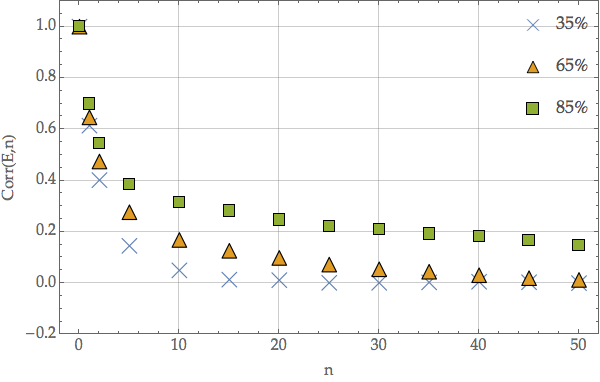
\includegraphics[width=\textwidth]{Figures/MCEnergyCorrelations}
	\caption[MC: Energy Correlation Series]{Energy correlation for a $4\times10^4$ equilibrated sample at $T=0.5$ and $\rho=0.35$. According to the acceptance ratio, the correlation length differs.}
	\label{fig:MCCorrSeries}
\end{figure}\\
To use nearly uncorrelated data for a meaningful quantity of interest with this setting, a sample distance of approximately $50$ MC-Steps is sufficient.
For the final estimate, the quantity with errors then resolves to
\begin{align}
	\begin{split}
	  \begin{array}{l l}
	  \overline{E}&=\hspace{0.2cm}\frac{1}{N}\sum\limits_{i=1}^N E_i\smallskip\\
	  	\Delta \overline{E}&=\hspace{0.2cm}\sqrt{\frac{1}{N-1}\sum\limits_{j=1}^{N}(\overline{E}-E_j)^2}
	  \end{array}
	  \hspace{1cm}\Braket{E} &=\overline{E} \pm \frac{\Delta E}{\sqrt N}.
	\end{split}
\end{align}
\medskip\\
In order to gain reasonable correlation trends, the samples have to be re\-corded in equilibrated states.
The time, until such a step is reached, depends on the temperature and density of the system - near the critical point of the phase diagramme, the convergence behaviour is worse than apart~(see Fig.~\ref{fig:MCEnergyConvergence}).
\begin{figure}[ht]
	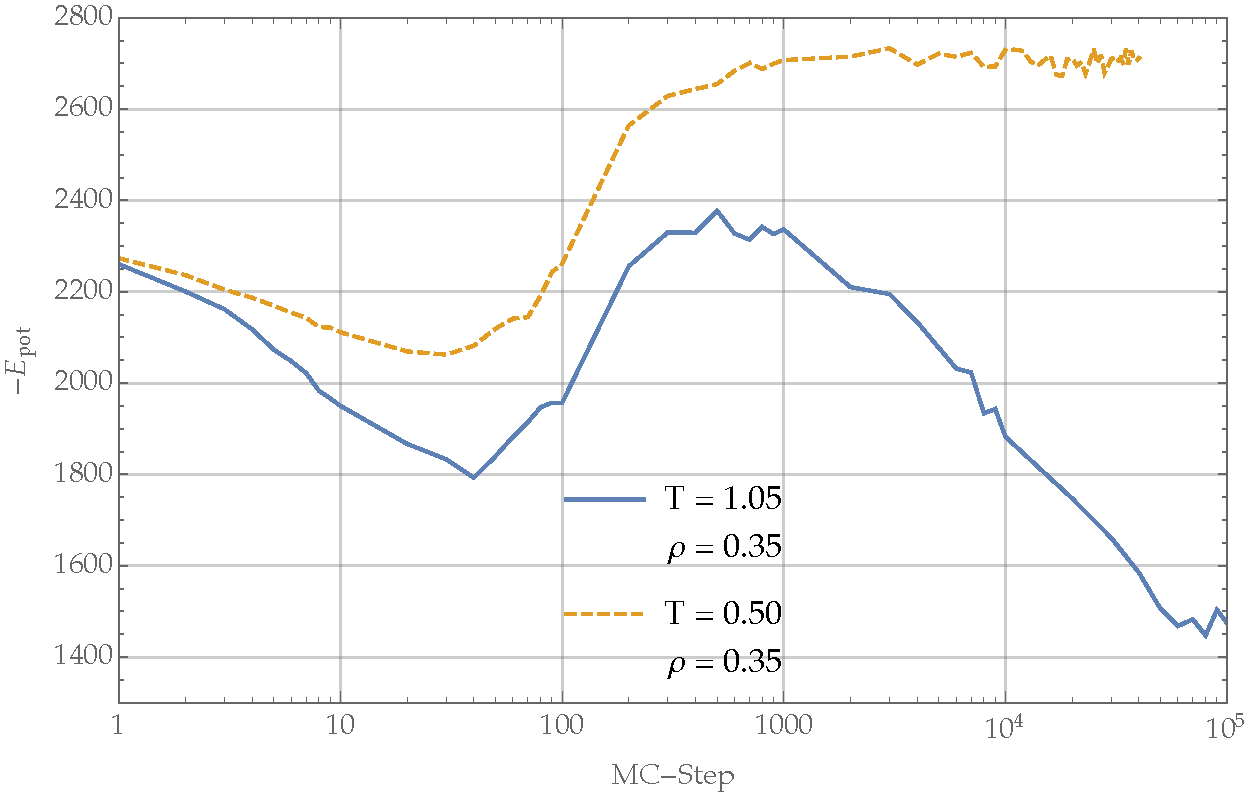
\includegraphics[width=\textwidth]{Figures/MCEnergyConvergence.pdf}
	\caption[MC: Energy Convergence Behaviour]{Energy convergence behaviour apart and near the critical point.}
	\label{fig:MCEnergyConvergence}
\end{figure}\\
Hence one has to analyse the correlation and convergence for each measurement in particular and decide which parameters are best, but due to time frame limitations, the setting is fixed and listed in Tab.~\ref{tbl:MCSettings}.
\begin{table}[ht]
	\centering
	\begin{tabular}{l | l}
		System specifics &Setting \\
		\hline
		Number of particles &chosen according to density and system size\\
		Acceptance ratio&roughly set $\approx$ \SI{60}{\percent}\\
		Equilibration&after $2\times10^5$ MC-Steps\\
		Quantity series&$6\times10^3$ samples with $150$ MC-Steps distance\\
	\end{tabular}
	\caption[MC: Settings]{Listing with settings for the measurement via Monte-Carlo.}
	\label{tbl:MCSettings}
\end{table}\\
The same considerations have been made in case for Molecular Dynamics, but the thermostat requires extra mentioning.

\section{Snapshots at Different Phase Points}
The typical phase diagramme of a Lennard-Jones potential near the critical point can be found in Fig.~\ref{fig:LJPhases}.
\begin{figure}[h!]
	\centering
	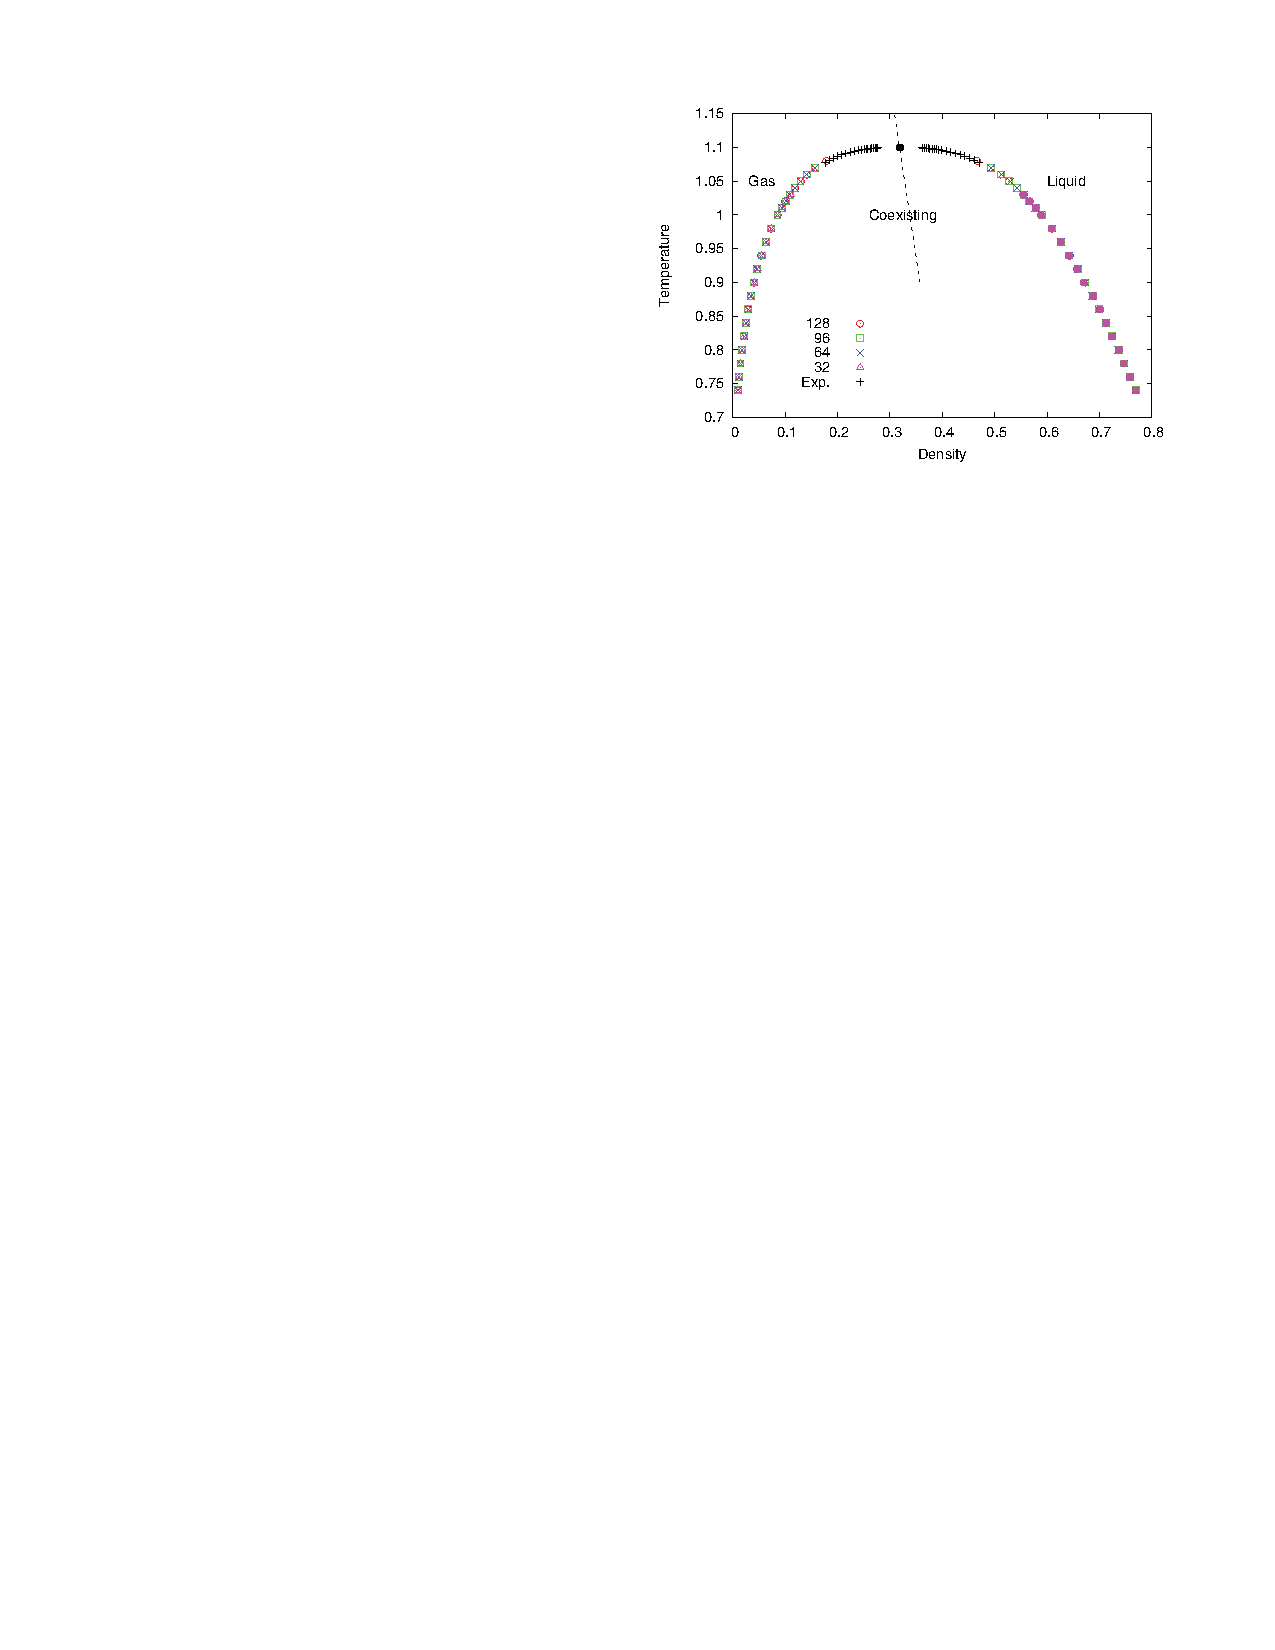
\includegraphics[width=0.6\textwidth]{LJPhases}
	\caption[LJ: Phase Diagramme]{The phase diagramme of a Lennard-Jones potential near the critical point~ZITIEREN!.}
\end{figure}
Hence after the system is in equilibrium, there can be found two phases - gaseous and liquid.
In principle, the function
\begin{align}
	\rho(z) = \frac{\rho_l - \rho_g}{2}\left(\tanh\left[(z_c-z)/lambda\right] + 1\right) + \rho_g
\end{align}
matches the density distribution and could be used to fit out the gaseous and liquid densities, respectively.
But for a simple and basic comparison, this reaches far beyond the scope of this work.
However, the next figure is an animation and shows snapshots of equilibrated states at different temperatures (Adobe Acrobat or similar PDF reader with java script support required).
\begin{figure}[h!]
	\centering
	\begin{minipage}[t]{\textwidth}
		\begin{minipage}[t]{0.4\textwidth}
			\centering
			\animategraphics[width=\textwidth,autoplay,loop,controls,buttonsize=1.2em]{0.5}{/animates/MCPhase}{1}{4}
		\end{minipage}
		\hspace{2cm}
		\begin{minipage}[t]{0.4\textwidth}
			\centering
			\animategraphics[width=\textwidth,autoplay,loop,controls,buttonsize=1.2em]{8}{/animates/MCPhaseSnapsT06}{0}{99}
		\end{minipage}
	\end{minipage}
	\caption[LJ Potential: Coexisting Phases at different temperatures]{Left: The coexisting phases mix together when the setting is close to the critical point.\\
	Right: 100 Frames show each step of an equilibrated state from the MC simulation.}
\end{figure}\\
For small densities and temperature, one can observe states resulting from the effects of PBC.
In explicit, these effects result in a droplet-liquid and a cylindrical-liquid phase, which can be seen in Fig.~\ref{fig:PBCPhases}.
\begin{figure}[ht]
	\centering
	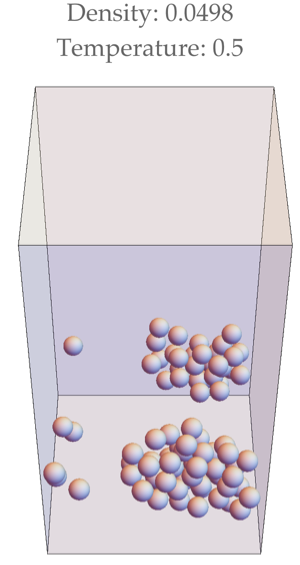
\includegraphics[width=0.3\textwidth]{MCDroplet}
	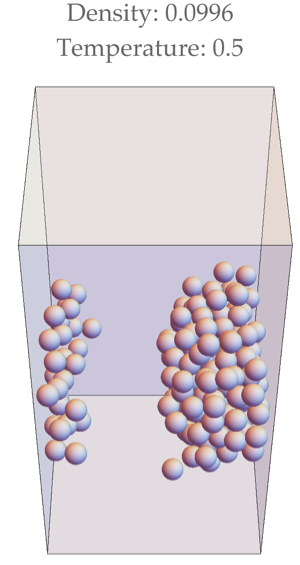
\includegraphics[width=0.3\textwidth]{MCCylinder}
	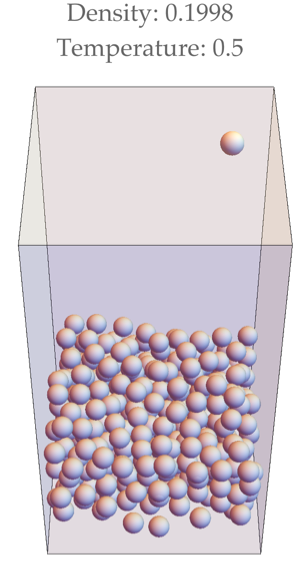
\includegraphics[width=0.3\textwidth]{MCCuboid}
	\caption[PBC: Phases Caused from Boundary Effects]{The phases shown above are caused from boundary effects.}
\end{figure}\\
Apart from side effects of PBC, perfect droplets are difficult to implement in a simulation, hence PBC are used to analyse droplet specifics e.g. surface tension.

\section{Conclusion}


%----------------------------------------------------------------------------------------
%	BIBLIOGRAPHY
%----------------------------------------------------------------------------------------

\renewcommand{\refname}{\spacedlowsmallcaps{References}} % For modifying the bibliography heading

\bibliographystyle{unsrt}

\bibliography{bibliography.bib} % The file containing the bibliography

%----------------------------------------------------------------------------------------

\end{document}
